%% Creator: Inkscape 1.3 (1:1.3+202307231459+0e150ed6c4), www.inkscape.org
%% PDF/EPS/PS + LaTeX output extension by Johan Engelen, 2010
%% Accompanies image file 'Lineare_antennen2.pdf' (pdf, eps, ps)
%%
%% To include the image in your LaTeX document, write
%%   \input{<filename>.pdf_tex}
%%  instead of
%%   \includegraphics{<filename>.pdf}
%% To scale the image, write
%%   \def\svgwidth{<desired width>}
%%   \input{<filename>.pdf_tex}
%%  instead of
%%   \includegraphics[width=<desired width>]{<filename>.pdf}
%%
%% Images with a different path to the parent latex file can
%% be accessed with the `import' package (which may need to be
%% installed) using
%%   \usepackage{import}
%% in the preamble, and then including the image with
%%   \import{<path to file>}{<filename>.pdf_tex}
%% Alternatively, one can specify
%%   \graphicspath{{<path to file>/}}
%% 
%% For more information, please see info/svg-inkscape on CTAN:
%%   http://tug.ctan.org/tex-archive/info/svg-inkscape
%%
\begingroup%
\makeatletter%
\providecommand\color[2][]{%
	\errmessage{(Inkscape) Color is used for the text in Inkscape, but the package 'color.sty' is not loaded}%
	\renewcommand\color[2][]{}%
}%
\providecommand\transparent[1]{%
	\errmessage{(Inkscape) Transparency is used (non-zero) for the text in Inkscape, but the package 'transparent.sty' is not loaded}%
	\renewcommand\transparent[1]{}%
}%
\providecommand\rotatebox[2]{#2}%
\newcommand*\fsize{\dimexpr\f@size pt\relax}%
\newcommand*\lineheight[1]{\fontsize{\fsize}{#1\fsize}\selectfont}%
\ifx\svgwidth\undefined%
	\setlength{\unitlength}{363.32178497bp}%
	\ifx\svgscale\undefined%
		\relax%
	\else%
		\setlength{\unitlength}{\unitlength * \real{\svgscale}}%
	\fi%
\else%
	\setlength{\unitlength}{\svgwidth}%
\fi%
\global\let\svgwidth\undefined%
\global\let\svgscale\undefined%
\makeatother%
\begin{picture}(1,1.16380096)%
	\lineheight{1}%
	\setlength\tabcolsep{0pt}%
	\put(0,0){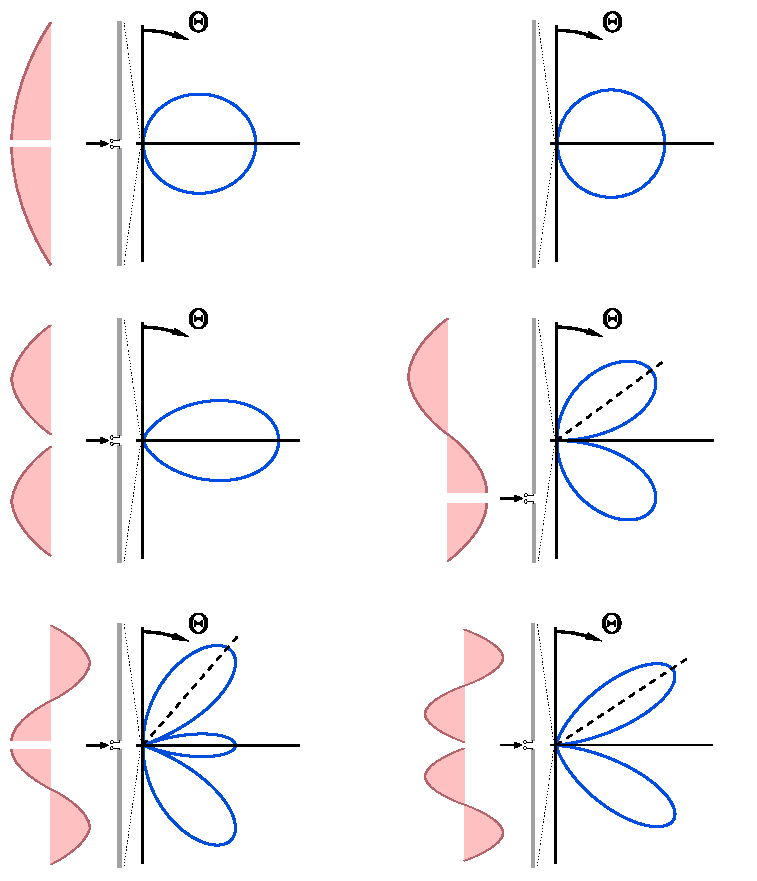
\includegraphics[width=\unitlength,page=1]{res/Lineare_antennen2.pdf}}%
	\put(-0.03749462,1.13927431){\color[rgb]{0,0,0}\makebox(0,0)[lt]{\lineheight{1.25}\smash{\begin{tabular}[t]{l}\textbf{Stomverteilung}\end{tabular}}}}%
	\put(0.21682177,1.05874075){\color[rgb]{0,0,0}\makebox(0,0)[lt]{\lineheight{1.25}\smash{\begin{tabular}[t]{l}\textbf{Fernfeld}\end{tabular}}}}%
	\put(0,0){\includegraphics[width=\unitlength,page=2]{res/Lineare_antennen2.pdf}}%
	\put(0.25016422,1.12146949){\color[rgb]{0,0,0}\makebox(0,0)[lt]{\lineheight{1.25}\smash{\begin{tabular}[t]{l}$\vartheta$\end{tabular}}}}%
	\put(0.24944189,0.72793128){\color[rgb]{0,0,0}\makebox(0,0)[lt]{\lineheight{1.25}\smash{\begin{tabular}[t]{l}$\vartheta$\end{tabular}}}}%
	\put(0.24899603,0.32657848){\color[rgb]{0,0,0}\makebox(0,0)[lt]{\lineheight{1.25}\smash{\begin{tabular}[t]{l}$\vartheta \quad 43^\circ$ \end{tabular}}}}%
	\put(0.79733669,1.12329457){\color[rgb]{0,0,0}\makebox(0,0)[lt]{\lineheight{1.25}\smash{\begin{tabular}[t]{l}$\vartheta$\end{tabular}}}}%
	\put(0.79595453,0.72835632){\color[rgb]{0,0,0}\makebox(0,0)[lt]{\lineheight{1.25}\smash{\begin{tabular}[t]{l}$\vartheta$\\$\quad\quad 54^\circ$\end{tabular}}}}%
	\put(0.78974511,0.32540434){\color[rgb]{0,0,0}\makebox(0,0)[lt]{\lineheight{1.25}\smash{\begin{tabular}[t]{l}$\vartheta$\\$\quad\quad\quad\quad 57^\circ$\\\end{tabular}}}}%
	\put(0.19493004,0.81773808){\color[rgb]{0,0,0}\makebox(0,0)[lt]{\lineheight{1.25}\smash{\begin{tabular}[t]{l}$\frac{\lambda}{2}$-Dipol\end{tabular}}}}%
	\put(0.19305147,0.42551962){\color[rgb]{0,0,0}\makebox(0,0)[lt]{\lineheight{1.25}\smash{\begin{tabular}[t]{l}$\lambda$-Dipol\end{tabular}}}}%
	\put(0.19487356,0.02299265){\color[rgb]{0,0,0}\makebox(0,0)[lt]{\lineheight{1.25}\smash{\begin{tabular}[t]{l}$\frac{3\lambda}{2}$-Dipol\end{tabular}}}}%
	\put(0.7386129,0.02186903){\color[rgb]{0,0,0}\makebox(0,0)[lt]{\lineheight{1.25}\smash{\begin{tabular}[t]{l}$2\lambda$-Dipol\end{tabular}}}}%
	\put(0.73937976,0.42576928){\color[rgb]{0,0,0}\makebox(0,0)[lt]{\lineheight{1.25}\smash{\begin{tabular}[t]{l}$\lambda$-Dipol\\(asymmetrische Sp.)\end{tabular}}}}%
	\put(0.73798866,0.81912619){\color[rgb]{0,0,0}\makebox(0,0)[lt]{\lineheight{1.25}\smash{\begin{tabular}[t]{l}Hertzscher Dipol\end{tabular}}}}%
	\put(0,0){\includegraphics[width=\unitlength,page=3]{res/Lineare_antennen2.pdf}}%
\end{picture}%
\endgroup%
